\section{Correction with entanglement}

\begin{figure}[ht!]
	\centering
	\begin{subfigure}[t]{0.49\linewidth}
		\centering
		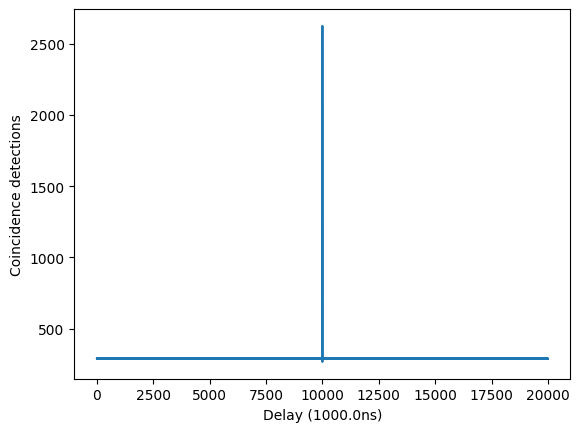
\includegraphics[height=4cm]{assets/unshifted_cc.png}
		\subcaption{}
	\end{subfigure}
	\begin{subfigure}[t]{0.49\textwidth}
		\centering
		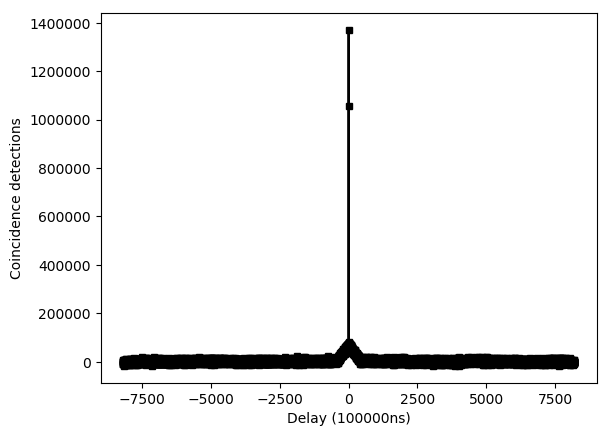
\includegraphics[height=4cm]{assets/firstDoppler_cc.png}
		\subcaption{}
	\end{subfigure}
	\caption{Autocorrelation of signal with (a) no shift (b) propagation delay}
	\label{fig:firstDoppler_cc}
\end{figure}
\begin{figure}[ht!]
	\centering
	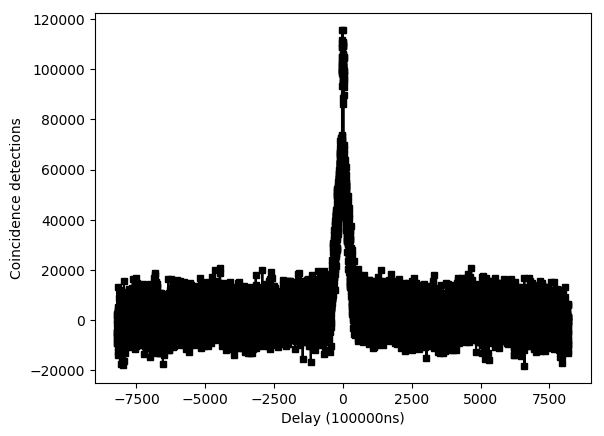
\includegraphics[width=0.95\linewidth]{assets/secondDoppler_cc.png}
	\caption{Autocorrelation of signal with delay and Doppler shift}
	\label{fig:secondDoppler_cc}
\end{figure}

\subsection{Ambiguity function}
The two-dimensional ambiguity function is commonly used in radar signal  analysis as the most complete statement of the waveform's inherent performance. It reveals the range-Doppler position of ambiguous responses and defines the range and Doppler resolution. It is defined as 

\begin{equation}
A(\nu,\tau)\equiv\int_{-\infty}^{\infty}\tilde{s}\big(t+\frac{\tau}{2}\big)\tilde{s}^*\big(t-\frac{\tau}{2}\big)e^{2i\pi\nu t} dt
\end{equation}

\subsection{Beat function}
In this case, a radio signal transmitted at a nominal frequency off0from a satellite in motion will appear at the receiver with aslightly different frequency offR.  This is significant because the amount of shift from thenominal frequency is mathematically related to the relative change in position of the satelliteover time.There are two methods by which GPS receivers typically measure this effect.  The firstand most common method arises simply from the way in which a GPS receiver maintainsits  satellite  locks.   It  has  been  shown  that  satellite  locks  are  achieved  by  maximizing  anautocorrelation  function  between  the  received  PRN  code  on  the  L1  signal  and  the  samelocally generated code shifted through time.  It is apparent that the autocorrelation functionmust be maximized by aligning the received and generated code sequences over a significantamount of time (at least one full code cycle).  This is only possible if the code being generatedhas the same frequency as the code being received.When  a  receiver  is  carrying  out  its  search-and-acquire  procedure  for  the  various  PRNcodes,  it  must  try  to  align  the  codes  not  only  in  time,  but  also  in  frequency.   As  such,most receivers will scale the generated code according to a set of frequency bins centeredaround the nominal L1 frequency [42].  Upon finding a frequency value (and alignment) thatresults in a successful autocorrelation, the frequency can then be fine-tuned to maximize theautocorrelation result.  The exact frequency that does so should be equal to the frequencyof  the  received  signal.   As  such,  the  instantaneous  Doppler  shift  can  be  found  by  simplysubtracting the nominal frequency from the received frequency:fD=fR−f0.14

It should be noted that the satellites and receivers are not moving relative to one anotherin a constant fashion; therefore, the Doppler shifts change over time.  The receiver is con-stantly tracking this shift to maintain its satellite lock, with the result that every Dopplerobservation is aninstantaneousobservation that changes with each consecutive epoch.The second method by which a receiver might calculate the Doppler shift to a satelliteis by determining thebeat frequencyresulting from mixing the received GPS signal with thelocally-generated one [5].  When two sine waves with slightly different frequencies are mixedtogether, a wave is produced with two frequency components equal to the sum and differenceof the original waves’ frequencies.  Knowing thatf≡dφ(t)dt, this can be written as:S1(t)⊗S2(t) =A1sin2πφ1(t)×A2sin2πφ2(t)=A1A22[cos2π(φ2(t)−φ1(t))−cos2π(φ2(t) +φ1(t))](3)By passing this resulting wave through a low-pass filter to remove the high-frequency com-ponent,  a  pure  sine  wave  containing  only  the  beat  frequency  (i.e.   the  Doppler  shift)  willremain:SB(t) =Bsin2πφB(t)(4)whereBis  the  amplitude  of  the  resulting  beat  signal  andφB(t)  is  the  resulting  phasedifference which changes as a function of time (a.k.a.  the beat frequency).  Once the Dopplershift  is  known,  it  can  be  used  to  determine  user  velocity,  signal  anomalies,  or  even  userposition with the aid of additional observables

\texttt{TODO: fill in machine learning method}

\begin{enumerate}
	\item find middle part with no shift
	\item try to shift middle part and find differential equation (order 2)
\end{enumerate}
 